\section{Machine learning}

\subsection{Environment}

In addition to the previous section's list of tools and libraries, we can mention \texttt{scikit-learn} whose SVM's implementation we use for our experiments. We also use its utility functions for data splitting and for metrics.

To define and train our neural networks, we use \texttt{keras} with \texttt{tensorflow} as the backend.

On our computing server, equipped with an NVidia GTX1070 graphics card, we use \texttt{tensorflow-gpu} to accelerate the calculations by using said graphics card.

% -------------------------------------------------------------------------------------------------------------
\subsection{Model architectures}

For all of the models described hereafter, we have made the input dimensions and the number of outputs modular. The goal is to be able to build different experiments easily and compare performance.

First, we use the Support Vector Machine (SVM) model provided by \texttt{sklearn} as a "control experiment". If the SVM's performance is as good or better than our more advanced models, we can worry that something is wrong. Either the problem is too easy, which probably means there are biases in the dataset, or our other models are not appropriate for the task.

Our first attempt at a Convolutional Neural Network (CNN) is based on the description in the work of \textcite{riyaz_deep_2018}. A representation of the layers is shown in figure \ref{fig:cnn-riyaz}. It achieved reasonable performance but was very prone to overfitting. Despite adding l2 regularization and increasing the dropout rate, this model still showed significant overfitting.

We later discovered that this was linked to the layer on which we performed the dropout operation. Indeed, it seems that in this situation, dropping out after the pooling layer, as opposed to doing it after the convolution layer, is a lot more effective. At this point, we had already started using the next CNN, which gave us slightly better results.

\begin{figure}[htbp!]
  \centering
  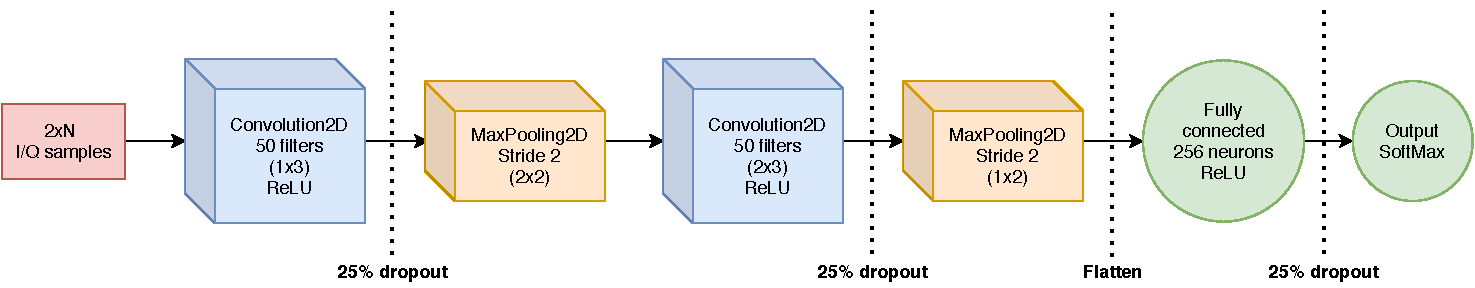
\includegraphics[scale=0.63]{figures/ml_riyaz.pdf}
  \caption{Representation of the first CNN used}
  \label{fig:cnn-riyaz}
\end{figure}

Said CNN is based on \textcite{youssef_machine_2017}'s description of their model. It is very similar to the previous one, but the convolution parameter seem more sensible and gave better results in our case. A representation of the model's layers is shown in figure \ref{fig:cnn-youssef}.

We tried adding an additional convolution layer to improve our accuracy but the performance boost was insignificant and of course it made the model slower to converge. The same applied when adding an additional dense layer. Increasing the number of neurons in the dense layer had a similar effect and also seemed to increase overfitting.

So it seems like this simple model is hard to improve upon. In the end, we added the dropout effect to the dense layer in addition to the pooling layers, in order to lower the tendency to overfit even more.

\begin{figure}[htbp!]
  \centering
  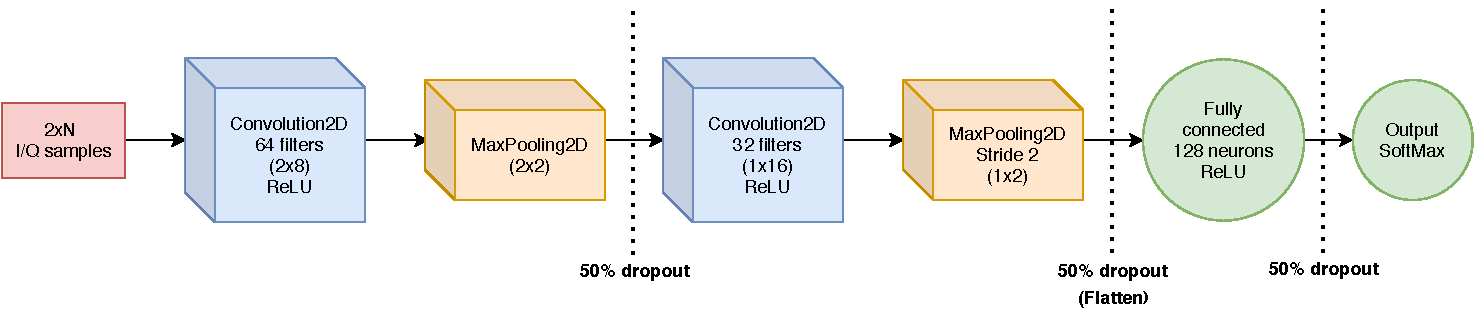
\includegraphics[scale=0.63]{figures/ml_youssef.pdf}
  \caption{Representation of the second CNN used}
  \label{fig:cnn-youssef}
\end{figure}

% -------------------------------------------------------------------------------------------------------------
\subsection{Default parameters}

Except if stated otherwise, the following experiments will use the model parameters listed in table \ref{tab:parameters}.

\begin{table}[htbp!]
  \centering
  \begin{tabular}{|l|l|}
    \hline
    \textbf{Parameter}             & \textbf{Value}            \\ \hline \hline
    \textbf{Window size}           & 512                       \\ \hline
    \textbf{Optimizer}             & Adam                      \\ \hline
    \textbf{Initial learning rate} & 0.001                     \\ \hline
    \textbf{Loss function}         & Categorical cross entropy \\ \hline
    \textbf{Batch size}            & 500                       \\ \hline
    \textbf{Number of epochs}      & 200                       \\ \hline
  \end{tabular}
  \caption{Default model parameters for our experiences}
  \label{tab:parameters}
\end{table}

% -------------------------------------------------------------------------------------------------------------
\subsection{Experiments with the first dataset}

no  find-peaks here

\subsubsection{Discriminating on chip type}

The first experiment we report on is about classifying tags from different types. To do so, we use tags 1, 6 and 9. The first is an NTAG213, the second a MiFare 1k and the last a FeliCa chip. Our SVM attained an accuracy of 69\%, and the confusion matrix is shown in figure \ref{fig:cmsvmchip}.

\begin{figure}[htbp!]
  \centering
  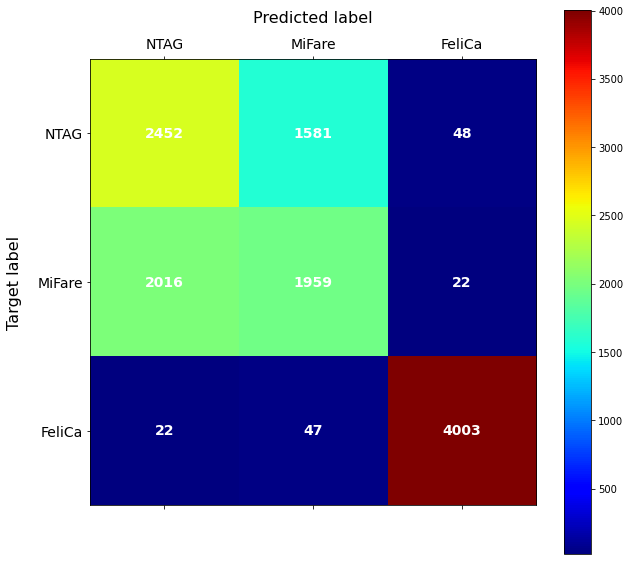
\includegraphics[scale=0.5]{figures/ml_svmchip512.png}
  \caption{Confusion matrix for the first experiment on SVM}
  \label{fig:cmsvmchip}
\end{figure}

As we had anticipated, discriminating between our NFC-A tags (the NTAG and the MiFare) and the FeliCa tag is trivial, but finding the difference between NFC-A tags is a lot more difficult. Here the SVM probably does little better than random guessing for the first two classes.

This experience is what motivated us not to include the FeliCa tag in the second dataset. It shows that its presence doesn't add any value to the experiments.

At this task, our CNN performed slightly better with an accuracy of 74\%. Its confusion matrix is shown in figure \ref{fig:cmcnnchip}.

\begin{figure}[htbp!]
  \centering
  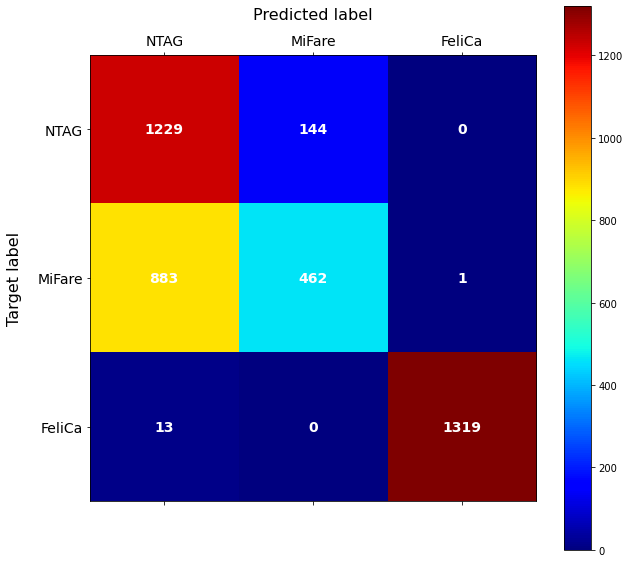
\includegraphics[scale=0.5]{figures/ml_cnnchip512.png}
  \caption{Confusion matrix for the first experiment on CNN}
  \label{fig:cmcnnchip}
\end{figure}

\subsubsection{Discriminating on tag}

Might not have enough information in signal...

% -------------------------------------------------------------------------------------------------------------
\subsection{Experiments with the more complete dataset}

SVM is unable to ...


plot performance per number of tags for svm and cnn


% -------------------------------------------------------------------------------------------------------------
\subsection{Reflection on the results}
